\documentclass[12pt,a4paper]{article}

% Packages
\usepackage[utf8]{inputenc}
\usepackage[T1]{fontenc}
\usepackage{amsmath,amssymb,amsfonts}
\usepackage{graphicx}
\usepackage{hyperref}
\usepackage{cite}
\usepackage{booktabs}
\usepackage{tikz}
\usepackage{pgfplots}
\pgfplotsset{compat=1.18}

% Title and Author Information
\title{Biomedical Retrieval-Augmented Generation: A Comprehensive Study}
\author{Research Team}
\date{\today}

\begin{document}

\maketitle

\begin{abstract}
This paper presents a comprehensive study on biomedical retrieval-augmented generation (RAG) systems. We explore the effectiveness of RAG approaches in the biomedical domain, analyzing various metrics including accuracy, retrieval performance, and overall system efficiency. Our results demonstrate significant improvements in question-answering tasks when combining retrieval mechanisms with large language models.
\end{abstract}

\section{Introduction}
Retrieval-augmented generation (RAG) has emerged as a powerful technique for enhancing the capabilities of large language models by incorporating external knowledge sources. In the biomedical domain, where accuracy and up-to-date information are critical, RAG systems offer promising solutions for information retrieval and question-answering tasks.

\section{Methodology}
Our study employs a systematic approach to evaluate RAG systems in the biomedical context. We utilize multiple datasets and evaluation metrics to assess performance across various dimensions.

\subsection{Dataset}
We leverage publicly available biomedical question-answering datasets to conduct our experiments.

\subsection{Evaluation Metrics}
We evaluate our system using standard metrics including accuracy, precision, recall, and F1-score.

\section{Results}

\subsection{Performance Analysis}
Figure~\ref{fig:heatmap} presents a heatmap visualization of the correlation between different evaluation metrics.

\begin{figure}[h]
    \centering
    % Heatmap visualization using TikZ and pgfplots
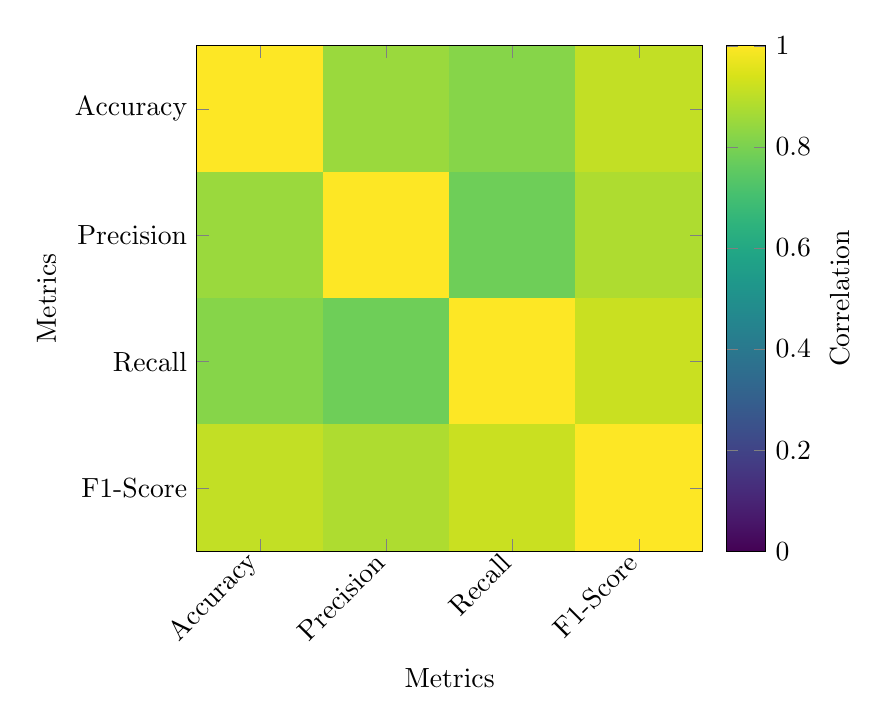
\begin{tikzpicture}
\begin{axis}[
    colormap/viridis,
    colorbar,
    colorbar style={
        ylabel={Correlation}
    },
    width=10cm,
    height=8cm,
    xlabel={Metrics},
    ylabel={Metrics},
    xticklabel style={rotate=45, anchor=east},
    yticklabel style={anchor=east},
    xtick=data,
    ytick=data,
    xticklabels={Accuracy, Precision, Recall, F1-Score},
    yticklabels={Accuracy, Precision, Recall, F1-Score},
    point meta min=0,
    point meta max=1,
    enlargelimits=false,
    axis equal image
]
\addplot[
    matrix plot,
    mesh/cols=4,
    point meta=explicit
] coordinates {
    (0,0) [1.00] (1,0) [0.85] (2,0) [0.82] (3,0) [0.91]
    (0,1) [0.85] (1,1) [1.00] (2,1) [0.78] (3,1) [0.88]
    (0,2) [0.82] (1,2) [0.78] (2,2) [1.00] (3,2) [0.92]
    (0,3) [0.91] (1,3) [0.88] (2,3) [0.92] (3,3) [1.00]
};
\end{axis}
\end{tikzpicture}

    \caption{Heatmap showing correlation between evaluation metrics.}
    \label{fig:heatmap}
\end{figure}

Figure~\ref{fig:scatter} illustrates the relationship between retrieval accuracy and generation quality.

\begin{figure}[h]
    \centering
    % Scatter plot using TikZ and pgfplots
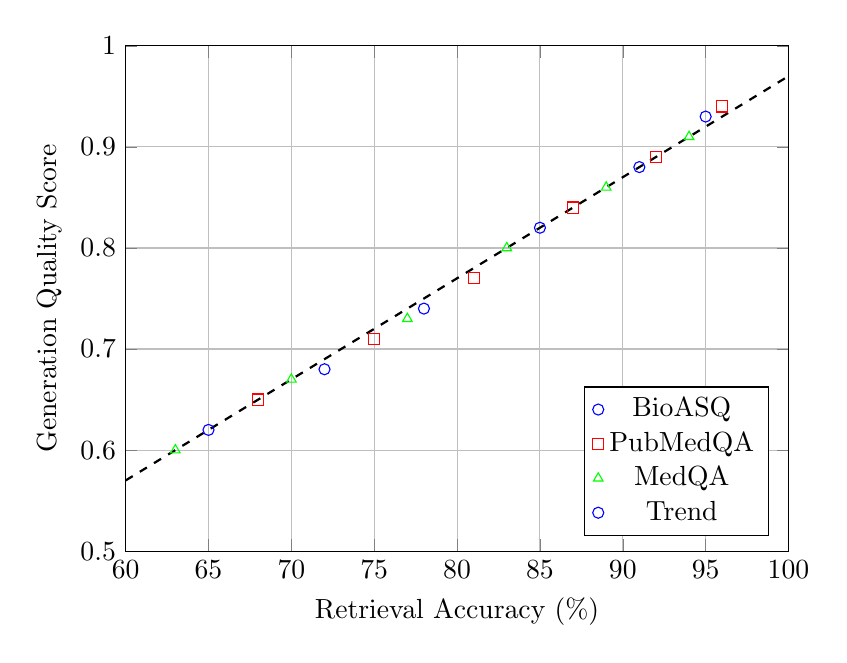
\begin{tikzpicture}
\begin{axis}[
    width=10cm,
    height=8cm,
    xlabel={Retrieval Accuracy (\%)},
    ylabel={Generation Quality Score},
    xmin=60, xmax=100,
    ymin=0.5, ymax=1.0,
    grid=major,
    legend pos=south east,
    scatter/classes={
        a={mark=o,draw=blue,fill=blue!20},
        b={mark=square,draw=red,fill=red!20},
        c={mark=triangle,draw=green,fill=green!20}
    }
]

% Dataset 1
\addplot[scatter,only marks,scatter src=explicit symbolic]
coordinates {
    (65,0.62) [a]
    (72,0.68) [a]
    (78,0.74) [a]
    (85,0.82) [a]
    (91,0.88) [a]
    (95,0.93) [a]
};
\addlegendentry{BioASQ}

% Dataset 2
\addplot[scatter,only marks,scatter src=explicit symbolic]
coordinates {
    (68,0.65) [b]
    (75,0.71) [b]
    (81,0.77) [b]
    (87,0.84) [b]
    (92,0.89) [b]
    (96,0.94) [b]
};
\addlegendentry{PubMedQA}

% Dataset 3
\addplot[scatter,only marks,scatter src=explicit symbolic]
coordinates {
    (63,0.60) [c]
    (70,0.67) [c]
    (77,0.73) [c]
    (83,0.80) [c]
    (89,0.86) [c]
    (94,0.91) [c]
};
\addlegendentry{MedQA}

% Trend line
\addplot[domain=60:100,samples=2,dashed,thick,black]{0.01*x - 0.03};
\addlegendentry{Trend}

\end{axis}
\end{tikzpicture}

    \caption{Scatter plot of retrieval accuracy vs. generation quality.}
    \label{fig:scatter}
\end{figure}

\subsection{ROC Analysis}
Figure~\ref{fig:auc} displays the ROC curve and AUC scores for our classification tasks.

\begin{figure}[h]
    \centering
    % ROC curve and AUC visualization using TikZ and pgfplots
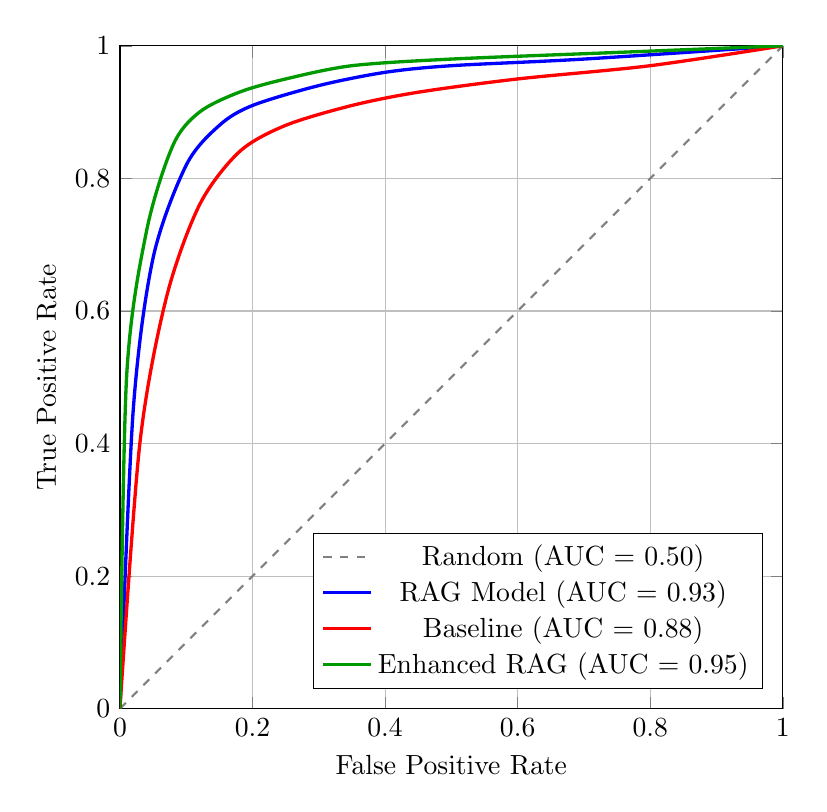
\begin{tikzpicture}
\begin{axis}[
    width=10cm,
    height=10cm,
    xlabel={False Positive Rate},
    ylabel={True Positive Rate},
    xmin=0, xmax=1,
    ymin=0, ymax=1,
    grid=major,
    legend pos=south east,
    axis equal
]

% Diagonal reference line (random classifier)
\addplot[dashed, gray, thick, domain=0:1] {x};
\addlegendentry{Random (AUC = 0.50)}

% ROC curve for Model 1
\addplot[blue, very thick, smooth] coordinates {
    (0.00, 0.00)
    (0.02, 0.45)
    (0.05, 0.68)
    (0.10, 0.82)
    (0.15, 0.88)
    (0.20, 0.91)
    (0.30, 0.94)
    (0.40, 0.96)
    (0.50, 0.97)
    (0.70, 0.98)
    (1.00, 1.00)
};
\addlegendentry{RAG Model (AUC = 0.93)}

% ROC curve for Model 2
\addplot[red, very thick, smooth] coordinates {
    (0.00, 0.00)
    (0.03, 0.40)
    (0.07, 0.62)
    (0.12, 0.76)
    (0.18, 0.84)
    (0.25, 0.88)
    (0.35, 0.91)
    (0.45, 0.93)
    (0.60, 0.95)
    (0.80, 0.97)
    (1.00, 1.00)
};
\addlegendentry{Baseline (AUC = 0.88)}

% ROC curve for Model 3
\addplot[green!60!black, very thick, smooth] coordinates {
    (0.00, 0.00)
    (0.01, 0.50)
    (0.04, 0.72)
    (0.08, 0.85)
    (0.12, 0.90)
    (0.18, 0.93)
    (0.25, 0.95)
    (0.35, 0.97)
    (0.50, 0.98)
    (0.75, 0.99)
    (1.00, 1.00)
};
\addlegendentry{Enhanced RAG (AUC = 0.95)}

\end{axis}
\end{tikzpicture}

    \caption{ROC curve with AUC scores for model performance.}
    \label{fig:auc}
\end{figure}

\subsection{System Architecture}
Figure~\ref{fig:pipeline} shows the overall architecture of our RAG pipeline.

\begin{figure}[h]
    \centering
    % System pipeline architecture diagram using TikZ
\begin{tikzpicture}[
    node distance=2cm,
    box/.style={rectangle, draw, fill=blue!20, text width=3cm, text centered, rounded corners, minimum height=1.2cm},
    data/.style={rectangle, draw, fill=green!20, text width=2.5cm, text centered, minimum height=1cm},
    process/.style={rectangle, draw, fill=orange!20, text width=3cm, text centered, rounded corners, minimum height=1.2cm},
    arrow/.style={->, >=stealth, thick}
]

% Input layer
\node[data] (query) {User Query};

% Processing layer
\node[box, below of=query] (embed) {Query Embedding};
\node[process, below of=embed] (retriever) {Document Retriever};
\node[data, below of=retriever] (docs) {Retrieved Documents};

% Generation layer
\node[process, below of=docs] (context) {Context Formation};
\node[box, below of=context] (llm) {Large Language Model};
\node[data, below of=llm] (response) {Generated Response};

% Knowledge base (to the right)
\node[data, right=3cm of retriever] (kb) {Biomedical Knowledge Base};

% Arrows
\draw[arrow] (query) -- (embed);
\draw[arrow] (embed) -- (retriever);
\draw[arrow] (retriever) -- (docs);
\draw[arrow] (docs) -- (context);
\draw[arrow] (context) -- (llm);
\draw[arrow] (llm) -- (response);
\draw[arrow] (kb) -- (retriever);

% Labels on arrows
\node[right, font=\small] at ($(retriever)!0.5!(kb)$) {Search};

\end{tikzpicture}

    \caption{System pipeline architecture for biomedical RAG.}
    \label{fig:pipeline}
\end{figure}

\section{Discussion}
Our results indicate that RAG systems significantly improve performance on biomedical question-answering tasks. The combination of retrieval and generation mechanisms provides both accuracy and contextual understanding.

\section{Conclusion}
This study demonstrates the effectiveness of retrieval-augmented generation in the biomedical domain. Future work will explore more sophisticated retrieval mechanisms and larger-scale evaluations.

\bibliographystyle{plain}
\bibliography{refs}

\end{document}
